\chapter{Klasifikácia pomocou siamskej neurónovej siete}
\label{kap:siamese}
V tejto kapitole popíšeme možnosti využitia siamskej neurónovej siete na problém rozpoznávania osôb.
Ukážeme dve riešenia tohto problému: rozpoznávanie podľa záberov tvárí a záberov celého tela.

\section{Siamská neurónová sieť}
Siamská neurónová sieť je typ neurónovej siete, ktorá je zložená z dvoch rovnakých podsietí. 
Tieto podsiete majú okrem architektúry aj rovnaké váhy v jednotlivých vrstvách.
Úlohou siamskej architektúry nie je priamo klasifikovať vstup.
Ich hlavné využitie je nájdenie podobnosti medzi dvomi vstupmi.
Hlavná myšlienka je založená na tom, že ak obe podsiete majú podobné vstupy, ich výstupné vektory budú blízko seba.
Naopak, ak sú vstupy málo podobné, výstupné vektory budú od seba ďalej.
Inak povedané, vstupy sú si podobné práve vtedy, keď je vzdialenosť medzi výstupnými vektormi malá.

\begin{figure}[H]
\centerline{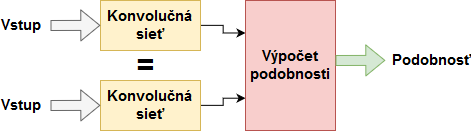
\includegraphics[width=0.8\textwidth]{images/siamese_diagram}}
\caption[Siamska neurónová sieť]{Jednoduchá architektúra siamskej neurónovej siete s konvolučnými podsieťami.}
\label{obr:siamese_diagram}
\end{figure}

Vzdialenosť \textit{d} medzi dvoma vektormi $p = (p_1, p_2, ..., p_n)$ a $q = (q_1, q_2, ..., q_n)$ 
môžeme merať viacerými spôsobmi. Uvádzame dve najpopulárnejšie metriky.

\begin{description}
\item[Manhattanovská vzdialenosť]
Vzdialenosť dvoch vektorov je súčet absolútnych hodnôt rozdielov ich kartézkych súradníc.
$$d(p, q) = \sum_{i=1}^{n} \| p_i - q_i \|$$

\item[Euklidovská vzdialenosť]
Vzdialenosť dvoch vektorov je dĺžka úsečky spájajúcej dva body reprezentované danými vektormi v n-rozmernom priestore.
$$d(p, q) = \sqrt{ \sum_{i=1}^{n} ( p_i - q_i )^2}$$
\end{description}


Obe uvedené metriky majú niekoľko dobrých vlastností.
\begin{description}
\item[Symetria] Dva vstupy sú si rovnako podobné bez ohľadu na to, do ktorej podsiete vstupujú. 
$$d(p, q) = d(q, p) $$
\item[Trojuholníková nerovnosť] Vysoká podobnosť vstupu s ďalšími dvomi vstupmi zaručí, že aj tieto vstupy si budú dostatočne podobné.
$$d(p, q) 	\leq d(p, z) + d(z, q)$$
\item[Nezápornosť a nulová vzdialenosť pre rovnaké vektory] Navzájom rovnaké vstupy dosahujú maximálnu podobnosť.
$$d(p, q) \geq 0$$
$$d(p, q) = 0 \Rightarrow p = q$$
\end{description}

\section{Klasifikácia}
Pri bežnej neurónovej sieti určenej priamo na klasifikáciu získame pre každý vstup triedu, do ktorej patrí.
V prípade klasifikácie osôb budú triedami napríklad ich mená.
Takýto prístup má niekoľko nevýhod.

Hlavným problémom je klasifikácia nových alebo neznámych osôb. 
Môžeme vytvoriť špeciálnu triedu, do ktorej budú patriť všetky neznáme osoby.
Ak však chceme klasifikovať viac ako jednu novú osobu a vyžadujeme, aby každá osoba bola zaradená do inej triedy, takáto trieda nám nepomôže.
Bude potrebné znova natrénovať sieť aj s novými osobami.
Takáto situácia môže nastať napríklad v podniku, ktorý sleduje prítomnosť svojich zamestnancov.
Pokiaľ firma zamestná nové osoby, bez opätovného trénovania siete ich nebude možné správne klasifikovať.
Existujú však situácie, kedy dopredu nevieme, aké a koľko osôb vlastne klasifikovať budeme a opätovné trénovanie siete teda nie je možné.

Ďalšou nevýhodou je, že aj pokiaľ sieť bude znova natrénovaná, na jej trénovanie je potrebný veľký počet záberov nových osôb, ktoré chceme klasifikovať.
Tieto zábery musia zachytávať nové osoby z rôznych uhlov a v rôznych polohách, čo v niektorých situáciách nemusí byť realizovateľné.

Klasifikácia pomocou siamskej neurónovej siete rieši všetky spomenuté problémy.
Po natrénovaní siete nám pre každú triedu stačí uchovávať len jeden vstup, ktorý do tejto triedy patrí a danú triedu reprezentuje.
Ak chceme vytvoriť novú triedu, opätovné trénovanie nie je potrebné, stačí len vytvoriť vstup, ktorý do tejto triedy patrí.

Klasifikácia prebieha jednoducho: ak je vstup, ktorý chceme klasifikovať, dostatočne podobný vstupu, ktorý reprezentuje niektorú triedu, bude aj tento vstup patriť do danej triedy.

\begin{figure}[H]
\centerline{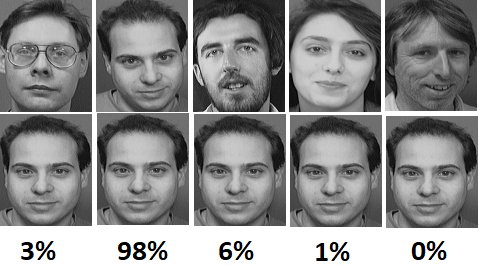
\includegraphics[width=1\textwidth]{images/oneshot_classification}}
\caption[Klasifikácia pomocou siamskej neurónovej siete]{Vrchný riadok reprezentuje jednotlivé triedy, do ktorých chceme klasifikovať, stredný riadok obsahuje záber, ktorý chceme klasifikovať a posledný riadok ukazuje percentuálnu zhodu v danom stĺpci.}
\label{obr:oneshot_classification}
\end{figure}

\section{Architektúra siete} \label{kap:siamese_architecture}
Oboje siete, na hľadanie podobnosti tvárí a na hľadanie podobnosti celých tiel, používajú tú istú architektúru.
Architektúra siete bola inšpirovaná sieťou určenou na klasifikáciu znakov v rôznych abecedách \cite{siamese_architecture}.
Vstupom do siete pre hľadanie podobnosti tvárí sú čiernobiele obrázky veľkosti 105x105 a 
do siete pre hľadanie podobnosti celých tiel sú farebné obrázky o veľkosti 65x155 s troma kanálmi farieb RGB.

Sieť obsahuje štyri konvolučné vrstvy, ktoré majú postupne 64, 128, 128 a 256 filtrov s veľkosťami kernelu 10x10, 7x7, 4x4 a 4x4.
Medzi nimi sa nachádzajú max pooling vrstvy, ktoré redukujú každú dimenziu na polovicu.
Max pooling funguje nasledovne: vstupnú maticu rozdelí na regióny rovnakej veľkosti (v našom prípade 2x2). 
Nová matica bude obsahovať len maximálne hodnoty v každom regióne.
Po každej max pooling vrstve nasleduje dropout s pravdepodobnosťou 15\% aby sme predišli preučeniu \cite{JMLR:v15:srivastava14a}. 
Ako aktivačné funkcie v konvolučných vrstvách využívame funkciu ReLU. 
Výstupom tejto funkcie je jej vstupný vektor, v ktorom sú všetky záporné hodnoty nahradené 0.

Po týchto vrstvách nasleduje plne-prepojená vrstva, jej výstupom je vektor o veľkosti 4096.
Takéto vektory vstupujú do ďalšej vrstvy dva, jeden z každej podsiete siamskej siete.
Vypočítame manhattanovskú vzdialenosť medzi nimi a výslednú vzdialenosť pretransformujeme pomocou sigmoid funkcie $S(x) = \frac{1}{1 + e^-x}$ na hodnoty z intervalu <0, 1>, 
kde jednotka značí maximálnu a nula minimálnu podobnosť vstupov do siete.

\begin{figure}[H]
\centerline{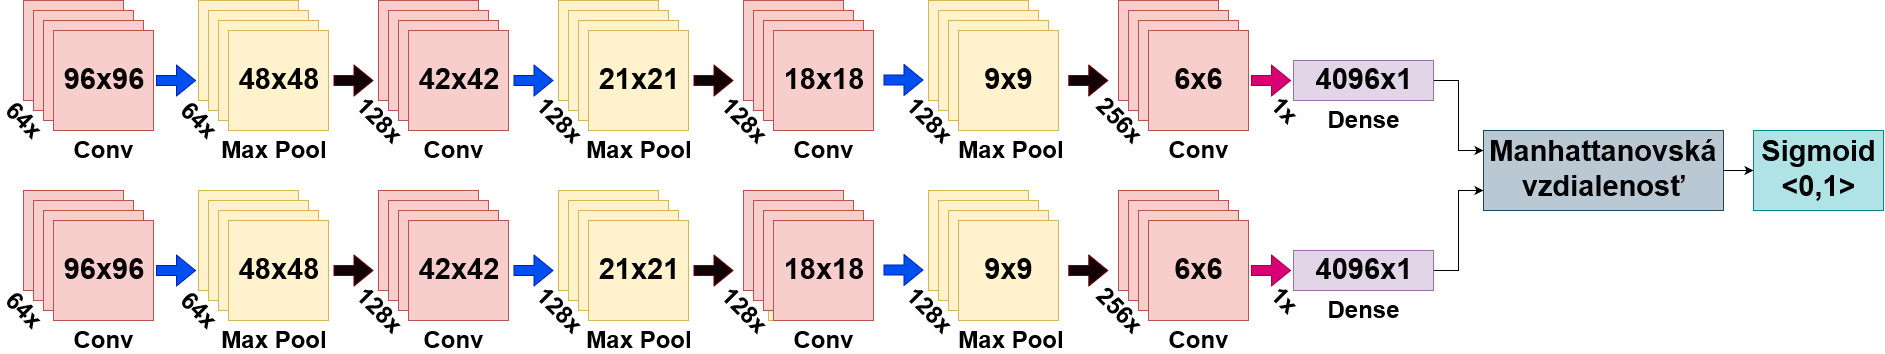
\includegraphics[width=1\textwidth]{images/siamese_architecture}}
\caption[Architektúra siete pre hľadanie podobností tvárí]{Ukážka jednotlivých vrstiev sieti pre hľadanie podobností tvárí}
\label{obr:siamese_architecture}
\end{figure}

\section{Trénovanie siete} \label{kap:siamese_train}
\subsection{Datasety}
Na trénovanie siete pre hľadanie podobnosti podľa snímok celých tiel sme opäť využili dataset DukeMTMC-reID \cite{ristani2016MTMC} \cite{zheng2017unlabeled} spomenutý v kapitole \ref{kap:features}.

Na hľadanie podobnosti tvárí sme zvolili iný dataset, pretože zábery v datasete DukeMTMC-reID nemajú dostatočné rozlíšenie na natrénovanie siete.
Vybrali sme dataset ChokePoint \cite{wong_cvprw_2011}. 
Tento dataset obsahuje zábery nasnímané v rozpätí jedného mesiaca pomocou trojíc kamier umiestnených na viacerých miestach.
Celkovo zachytáva 29 rôznych identít na celkovo 64 204 snímkach ich tvárí.
Zábery sme rozdelili na trénovaciu a testovaciu množinu.
Tri osoby sa vyskytujú len v testovacej množine rovnako ako všetky zábery z niektorých zvolených kamier.
Trénovacia množnina celkovo obsahuje 11 323 snímok, trénovacia 52 247 snímok.

\begin{figure}[H]
\centerline{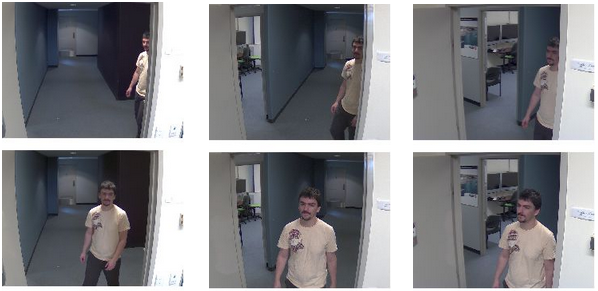
\includegraphics[width=1\textwidth]{images/chokepoint_same}}
\caption[Ukážka datasetu]{Zábery jednej osoby z jednej trojice kamier v datasete ChokePoint}
\label{obr:choke_same}
\end{figure}

\subsection{Stratová funkcia}
Ako stratovú funkciu sme zvolili binárku cross entropiu medzi predikciami a očakávanými hodnotami.
Formálne, chybová funkcia L je definovaná:
$$L(p, q) = t(p, q) * log(s(p, q)) + (1 - t(p, q)) * log(1 - s(p, q))$$
\[
  t(p, q) =
  \begin{cases}
    1 & \text{ak p a q patria do rovnakej triedy} \\
    0 & \text{inak}
  \end{cases}
\]
$$s(p, q) = predikcia\ podobnosti$$
Vyskúšali sme použiť aj kontrastnú stratu L`.
$$L`(p, q) = \frac{1}{2} * t(p, q) * max(0, m - D(p, q))^2 + \frac{1}{2}*(1 - t(p, q)) * D(p, q)^2$$
\[
  t(p, q) =
  \begin{cases}
    1 & \text{ak p a q patria do rovnakej triedy} \\
    0 & \text{inak}
  \end{cases}
\]
$$D(p, q) = predikcia\ vzdialenosti$$
$$m = hyperparameter$$
Dosiahnuté výsledky pri učení však boli v porovnaní s cross entropiou výrazne horšie po rovnakej časovej dobe učenia.
Výhodou cross entropie je v tomto prípade aj to, že nemusí vhodne voliť žiaden hyperparameter.

Na minimalizáciu chyby sme použili optimalizátor Adam s rýchlosťou učenia len 0,001.
Vyššie hodnoty spôsobovali príliš veľké kolísanie chyby medzi jednotlivými iteráciami, čo paradoxne spôsobilo pomalšie učenie.

\subsection{Popis trénovania}
Trénovanie prebiehalo v 25\,000 iteráciách v prípade hľadania podobnosti tvárí a v 60\,000 iteráciách v prípade hľadania podobnosti celých tiel.
V každej iterácii sme zvolili osem osôb.
Pre každú osobu bol zvolený jeden náhodný záber.
Následne sme z každej kamery sme vybrali jeden záber, ktorý zachytáva tú istú osobu a jeden záber, ktorý zachytáva inú osobu.
Pokiaľ sa rovnaká osoba na tejto kamere nenachádzala, nevybrali sme ani záber inej osoby, aby zostal pomer rovnakých a rôznych osôb rovnaký.

Prvý zvolený záber bol porovnávaný s každým vybraným záberom tej istej osoby, pričom očakávaná hodnota podobnosti mala byť 1.
Rovnako bol porovnávaný s každým vybraným záberom iných osôb s očakávanou hodnotou podobnosti 0.

\begin{figure}[H]
\centerline{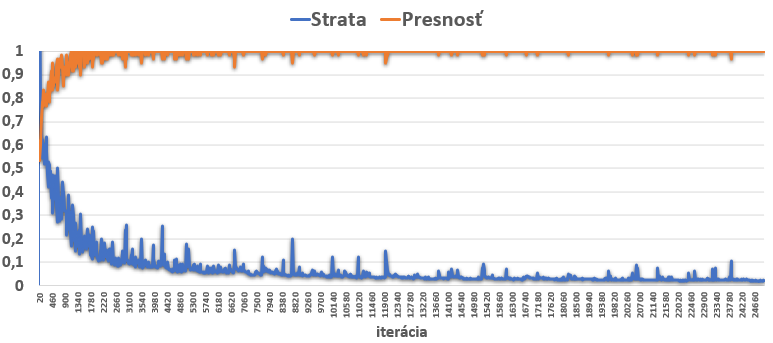
\includegraphics[width=1\textwidth]{images/graph_learn_face.png}}
\caption[Priebeh učenia hľadania podobnosti tvárí]{Priebeh učenia hľadania podobnosti tvárí. Z grafu vidieť, že na natrénovanie siete stačí aj menší počet iterácií na dosiahnutie dobrej presnosti.}
\label{obr:graph_learn_face}
\end{figure}

\begin{figure}[H]
\centerline{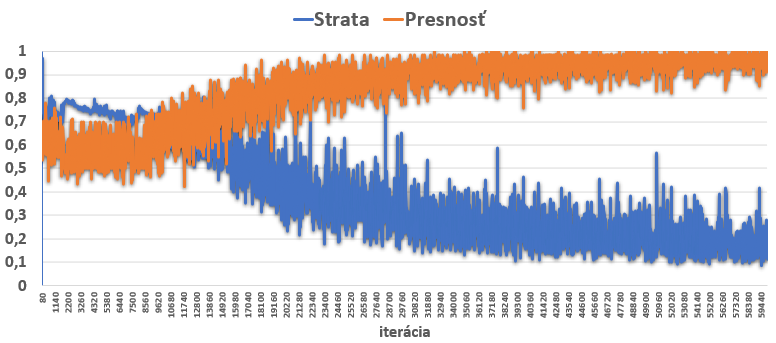
\includegraphics[width=1\textwidth]{images/graph_learn_body.png}}
\caption[Priebeh učenia hľadania podobnosti tiel]{Priebeh učenia hľadania podobnosti tiel. Na natrénovanie je potrebný väčší počet iterácií, ale sieť dosahuje dobrú presnosť na trénovacích príkladoch.}
\label{obr:graph_learn_body}
\end{figure}


\section{Výsledky}

\subsection{Meranie úspešnosti}
Kvalitu siete ukážeme pomocou chybovej tabuľky, ktorá má dva stĺpce a dva riadky, zobrazujúcej
správne zhody, nesprávne zhody, správne nezhody a nesprávne nezhody na náhodne vybraných dvojiciach obrázkov \cite{roc}.

\begin{description}
\item[Správna zhoda (TP)]
Snímky na vstupe patria rovnakej osobe a sieť rozhodla správne (podobnosť bola vysoká).

\item[Nesprávna zhoda (FP)]
Sieť rozhodla, že snímky na vstupe patria rovnakej osobe, avšak v skutočnosti zachytávajú rôzne osoby

\item[Správna nezhoda (TN)]
Snímky na vstupe nepatria rovnakej osobe a sieť rozhodla správne (podobnosť bola nízka).

\item[Nesprávna nezhoda (FN)]
Sieť rozhodla, že snímky na vstupe zachytávajú rôzne osoby, no v skutočnosti patri tej istej osobe.
\end{description}

Z týchto hôdnot odvodíme ďalšie hodnoty, ktoré dobre ukazujú kvalitu siete.

\begin{description}
\item[Presnosť (ACC)] Pravdepodobnosť správneho rozhodnutia siete na ľubovoľných príkladoch.
$$ACC = \frac{TP + TN}{TP + FP + TN + FN}$$
\item[Senzitivita (TPR)] Pravdepodobnosť správneho rozhodnutia na príkladoch, na ktorých vstupné snímky patrili rovnakej osobe.
$$TPR = \frac{TP}{TP + FN}$$
\item[Špecificita (TNR)] Pravdepodobnosť správneho rozhodnutia na príkladoch, na ktorých vstupné snímky nepatrili rovnakej osobe.
$$TNR = \frac{TN}{TN + FP}$$
\item[Precíznosť (PPV)] Pomer správnych rozhodnutí na príkladoch, na ktorých vstupné snímky patrili rovnakej osobe, k počtu rozhodnutí, v ktorých sieť určila, že vstupné snímky patrili rovnakej osobe.
$$PPV = \frac{TP}{TP + FP}$$
\item[Negatívna predikčná hodnota (NPV)] Pomer správnych rozhodnutí na príkladoch, na ktorých vstupné snímky nepatrili rovnakej osobe, k počtu rozhodnutí, v ktorých sieť určila, že vstupné snímky nepatrili rovnakej osobe
$$NPV = \frac{TN}{TN + FN}$$
\end{description}

Následne vyskúšame priamo klasifikovať osobu.
Každá trieda bude reprezentovať inú osobu len jedným záberom.
Vyberie jednu z týchto osôb a nejaký iný záber tejto osoby a tento záber porovnáme so zábermi každej triedy.
Osobu klasifikujeme do triedy s najväčšou podobnosťou.

\subsection{Výsledky pre hľadanie podobnosti tvárí}

Na testovacej databáze záberov tvárí sme dosiahli dobré výsledky vzhľadom na precíznosť a špecificitu.
Ak sieť určí, že vstupné snímky patria rovnakej osobe, s pravdepodobnosťou viac ako 92\% je to pravda.
Rovnako, ak snímky nezachytávajú rovnakú osobu, sieť s pravdepodobnosťou až 95\% spraví správne rozhodnutie.
Hlavným problémom sa ukazujú falošné nezhody.
Ak je na záberoch rovnaká osoba, sieť spraví správne rozhodnutie len v 59\% prípadov.

Pri testovaní sme vyhodnotili zhodu, ak výstupná hodnota siete bola väčšia ako 0,5. 
Ak by sme chceli znížiť počet falošných nezhôd a nevadia nám falošné zhody, je túto hodnotu možné znížiť.


\begin{table}[H]
  \caption[Úspešnosť hľadania podobnosti tvárí]{Úspešnosť hľadania podobnosti tvárí bez akéhokoľvek zmenšovania.}
  \label{tbl:face1_table}
  \begin{center}
  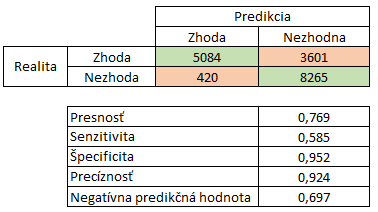
\includegraphics{images/face1_table}
  \end{center}
\end{table}

Výsledky klasifikácie do tried sme porovnali s modelom, ktorý vstup klasifikuje do náhodnej triedy.

\begin{figure}[H]
\centerline{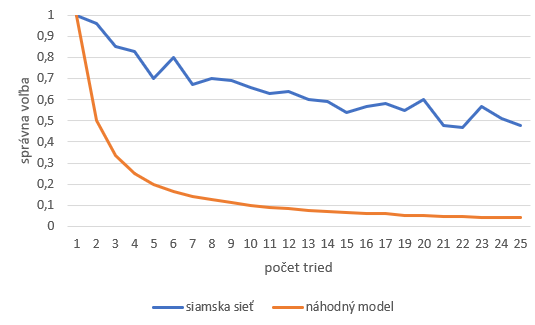
\includegraphics[width=1\textwidth]{images/graph_oneshot_face.png}}
\caption[Výsledky klasifikácie podľa tváre]{Graf porovnáva úspešnosť klasifikácie pomocou siamskej siete s náhodným modelom pre rôzne počty klasifikačných tried.}
\label{obr:graph_oneshot_face}
\end{figure}


Následne sme vyskúšali hľadanie podobnosti aj na záberoch tvárí s menším rozlíšením.
Zábery v testovacom datasete sme zmenšili na tretinu v oboch rozmeroch a sledovali sme, či sa zmení presnosť.
Keďže trénovanie prebiehalo len na záberoch v rovnakom rozlíšení, sieť sa mohla preučeniť na danom rozlíšení a presnosť sa mohla výrazne znížiť.
Zmena v meraných hodnotách však bola zanedbateľná.
Ak by však zmena nastala, jednoduchým riešením by bolo sieť znova natrénovať na rovnakých záberoch, ktoré by sme náhodne zmenšovali.



\begin{table}[H]
  \caption[Úspešnosť hľadania podobnosti tvárí na zmenšených snímkach]{Úspešnosť hľadania podobnosti tvárí na zmenšených snímkach.}
  \label{tbl:face1_table}
  \begin{center}
  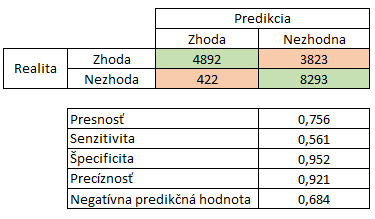
\includegraphics{images/face2_table}
  \end{center}
\end{table}

\begin{figure}[H]
\centerline{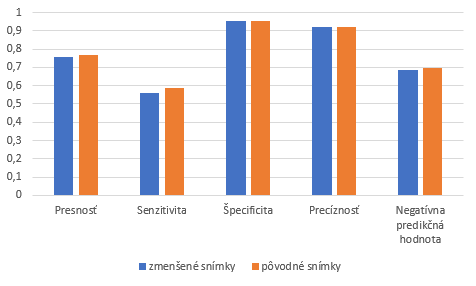
\includegraphics[width=0.9\textwidth]{images/graph_face12_compare.png}}
\caption[Porovnanie hľadania podobnosti tvárí na snímkach pôvodnej a zmenšenej veľkosti]{Graf porovnáva hľadanie podobnosti tvárí na snímkach pôvodnej a zmenšenej veľkosti.}
\label{obr:graph_face12_compare}
\end{figure}


\subsection{Výsledky pre hľadania podobnosti tiel}
Pri hľadania podobnosti tiel sme dosiahli podobné výsledky ako pri hľadania podobnosti tvárí.
Dosahujeme však menší počet falošných nezhôd.
\begin{table}[H]
  \caption[Úspešnosť hľadania podobnosti tiel]{Úspešnosť hľadania podobnosti tiel.}
  \label{tbl:body1_table}
  \begin{center}
  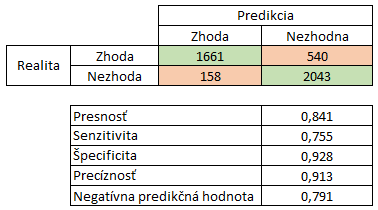
\includegraphics{images/body1_table}
  \end{center}
\end{table}

Výsledky klasifikácie do tried sme taktiež porovnali s modelom, ktorý vstup klasifikuje do náhodnej triedy.

\begin{figure}[H]
\centerline{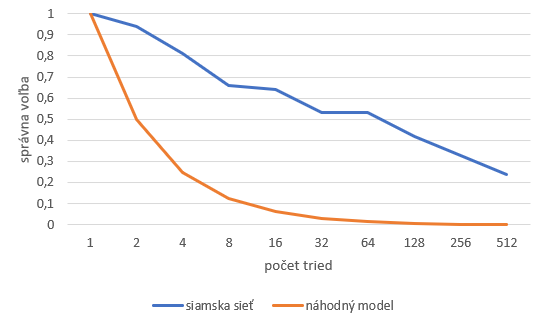
\includegraphics[width=1\textwidth]{images/graph_oneshot_body.png}}
\caption[Výsledky klasifikácie podľa tela]{Graf porovnáva úspešnosť klasifikácie pomocou siamskej siete s náhodným modelom pre rôzne počty klasifikačných tried.}
\label{obr:graph_oneshot_body}
\end{figure}

\subsection{Diskusia}
Z dosiahnutých výsledkov môžeme povedať, že oboje riešenia sa dajú využiť v systéme na sledovanie osoby vo viacerých záznamoch.
Problémom, ktorý treba vyriešiť, však zostávajú falošné nezhody, ktoré sú pri prechode osoby medzi zábermi dvoch kamier a jej následnej reidentifikácii dôležité.
Ich elimináciou by sme docielili správnu reidentifikáciu osoby na druhom zázname.
Riešením by mohla byť kombinácia riešení navrhnutých v tejto kapitole.
